\section{Introduction}
Over the past two decades, major advances have been made in estimating structured parameters, e.g., sparse, low-rank, etc., in high-dimensional small sample problems \cite{candes2010power, donoho2006compressed, friedman2008sparse}. Such estimators consider a suitable (semi) parametric model of the response: $y = \phi(\x,\bbeta^*) + w$ based on $n$ samples $\{(\x_i,y_i)\}_{i=1}^n$ and the parameter of interest, $\bbeta^* \in \reals^p$. The unique aspect of such high-dimensional regime of $n \ll p$ is that the structure of $\bbeta^*$ makes
the estimation possible for large enough samples $n = m$ known as the sample complexity \cite{candes2009exact, candes2006robust, tibshirani1996regression}. While the earlier developments in such high-dimensional estimation problems had focused on parametric linear models, the results have been widely extended to non-linear models, e.g., generalized linear models \cite{bach2012optimization, negahban2009unified}, broad families of semi-parametric and single-index models \cite{boufounos20081, plan2017high}, non-convex models \cite{blumensath2009iterative,jain2013low}, etc.

In several real world problems, the assumption that one global model parameter $\bbeta_0^*$ is suitable for the entire population is unrealistic.
We consider the more general setting where the population consists of sub-populations (groups) which are similar is many aspects but have unique differences. For example, in the context of anti-cancer drug sensitivity prediction where the goal is to predict responses of different tumor cells to a drug, using a same prediction model across cancer types (groups) ignores the unique properties of each cancer and leads to an uninterpretable global model. Alternatively, in such a setting, one can assume a separate model for each group $g$ as $y = \phi(\x, \bbeta_g^*) + w$ based on a group specific parameter $\bbeta^*_g$. Such a modeling choice fails to leverage the similarities across the sub-populations, and can only be estimated when sufficient number of samples are available for each group which is not the case in several problems, e.g., anti-cancer drug sensitivity prediction \cite{barretina2012cancer, iorio2016landscape1}.

The middle ground model for such a scenario is the \emph{superposition} of common and individual parameters $\bbeta_0^* + \bbeta_g^*$ which has been of recent interest \cite{??, guba16}. Such a collection of \emph{coupled} superposition models is known by multiple names in the statistical machine learning community. It is a form of multi-task learning \cite{jrsr10, Zhang2017-rm} when we consider regression in each group as a task. It is also called data sharing \cite{grti16} since information contained in different groups is shared through the common parameter $\bbeta_0^*$. And finally, it has been called data enrichment \cite{Chen2015-fj} because we enrich our data set with pooling multiple samples from different but related sources. 

Following the successful application of such a modeling scheme in recent years \cite{domu16, grti16,  olvi14, olvi15}, we consider the below \emph{data enrichment} (DE) model: 
\be
\label{eq:dsl}
y_{gi} &=& \phi(\x_{gi}, (\bbeta_0^* + \bbeta^*_g)) + w_{gi}, \quad g \in \{1, \dots, G\}~,
\ee
where $g$ and $i$ index the group and samples respectively. 
\begin{figure}%[!b]
	\centering
	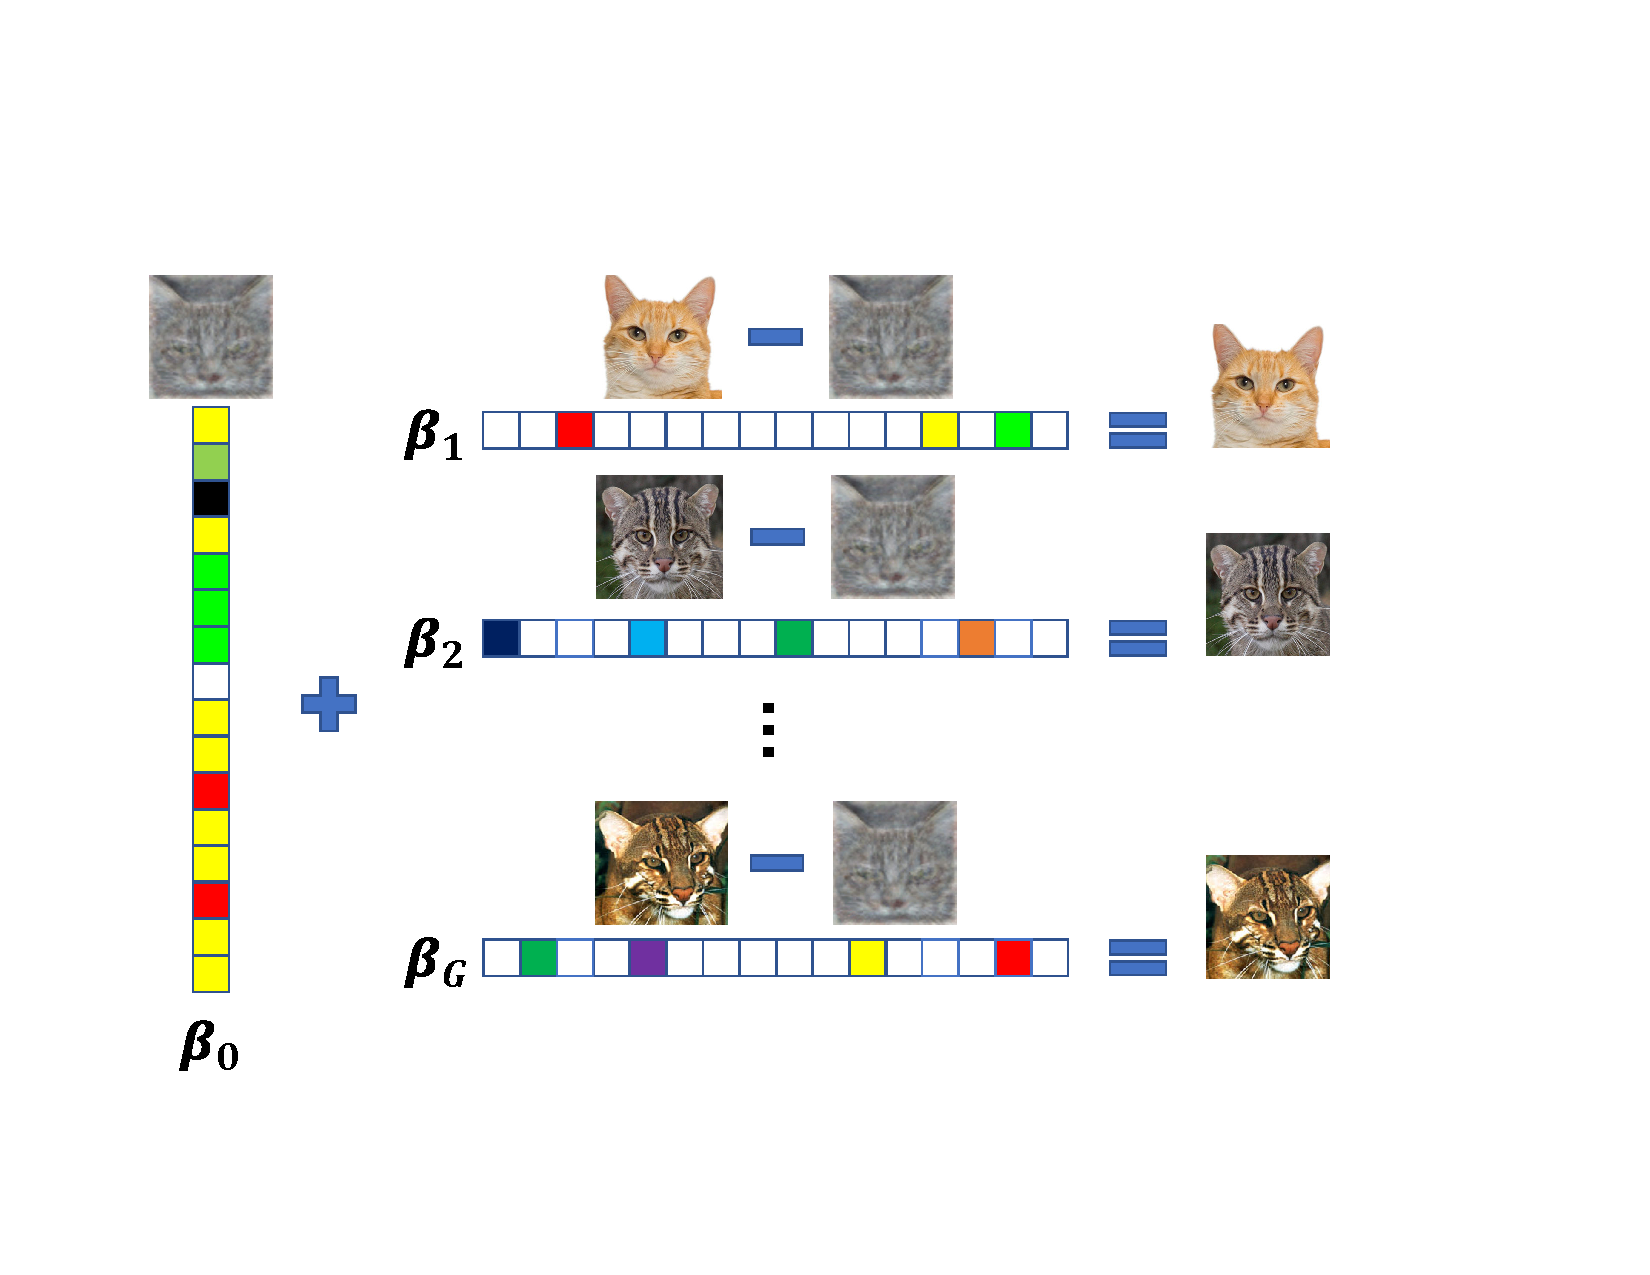
\includegraphics[scale=.45]{./img/concept.pdf}
	\caption{A conceptual illustration of data enrichment model for learning representation of  cat species. The common parameter $\bbeta_0$ captures a \emph{generic cat} which consists of shared features among all cats.}
	\label{fig:cat}		
\end{figure}
DE model \eqref{eq:dsl} assumes that there is a \emph{common} parameter $\bbeta^*_0$ shared between all groups which models similarities between all samples. And there are \emph{individual} per-group parameters $\bbeta_g^*$s each characterize the deviation of group $g$, Figure \ref{fig:cat}.% and capture unique aspects of each group.

\paragraph{The setting} Our goal is to design an estimation procedure which consistently recovers all parameters of DE \eqref{eq:dsl} fast and with small number of samples.
We specifically focus on the high-dimensional small sample regime where the number of samples $n_g$ for each group is much smaller than the ambient 
dimensionality, i.e., $\forall g: n_g \ll p$. Similar to all other high-dimensional models, we assume that the parameters $\bbeta_g$ are structured, i.e., for suitable convex functions $f_g$'s, $f_g(\bbeta_g)$ is small.
For example, when the structure is sparsity, $f_g$s are $L_1$-norms. Further, for the technical analysis and proofs,
we focus on the case of linear models, i.e., $\phi(\x,\bbeta) = \x^T \bbeta$. The results
seamlessly extend to more general non-linear models, e.g., generalized linear models, broad families of semi-parametric and single-index models, non-convex models, etc., using
existing results, i.e., how models like LASSO have been extended to these settings \cite{negahban2012restricted}. %(e.g.~employing ideas such as restricted strong convexity ). %{\color{red}{it is OK I think}}\ab{Is the last line correct? Lets check this.}

%We call these set of models, \emph{``data sharing''} model \cite{grti16}.
%In high dimensional regime, we assume that both common and individual parameters are structured, i.e., for suitable \emph{convex} functions $f_g$, $f_g(\bbeta^*_g)$s are small.
% and one desirable scenario is when the common parameter is much denser than the individual ones.
%In other words, for $g \in \{1, \dots, G\}$ $\bbeta^*_g$s are $s_g$-sparse vectors where $s_0 \gg s_g$.
%The common parameter $\bbeta^*_0$ captures the shared effect of features among groups.
%the ``dense similarity'' and individual parameters capture ``slight difference'' between groups and hopefully common parameter estimation will benefit from all of the shared data.

\subsection{Related Work}
In the context of \emph{Multi-Task Learning} (MTL), similar models have been proposed which have the general form of $y_{gi} = \x_{gi}^T (\bbeta_{1g}^* + \bbeta^*_{2g}) + w_{gi}$ where $\B_1 = [\bbeta_{11}, \dots, \bbeta_{1G}]$ and $\B_2 = [\bbeta_{21}, \dots, \bbeta_{2G}]$ are two parameter matrices \cite{Zhang2017-rm}. To capture the relation of tasks, different types of constraints are assumed for parameter matrices. For example, \cite{Chen2012-fb} assumes $\B_1$ and $\B_2$ are sparse and low rank respectively. In this parameter matrix decomposition framework for MLT, the most related work to ours is the Dirty Model (DM) proposed in \cite{jrsr10} where authors regularize the regression with $\norm{\B_1}{1, \infty}$ and $\norm{\B_2}{1,1}$ where norms are $p,q$-norms on \emph{rows} of matrices, i.e., $\norm{\cdot}{p,q} = \norm{(\norm{\cdot}{q}, \dots, \norm{\cdot}{q})}{p}$. 

If in our DE model we pick all structure inducing functions $f_g$ to be $l_1$-norm, the resulting model is very similar to the DM where $\norm{\B_1}{1, \infty}$ induces similarity between tasks and $\norm{\B_2}{1,1}$ models their discrepancies. On the other hand, the degree of freedom of DM model is higher than DE because $\norm{\B_1}{1, \infty}$ regularizer enforces shared support of $\bbeta^*_{1g}$s, i.e., $\text{supp}(\bbeta_{1i}^*) = \text{supp}(\bbeta_{1j}^*)$ but allows $\bbeta_{1i}^* \neq \bbeta_{1j}^*$ while in DE we have a single common parameter $\bbeta_0^*$. So one would expect that DE estimators should have smaller sample complexity compared to their DM counterparts and our analysis confirm that our estimator is more data efficient than DM estimator of \cite{jrsr10}. Mainly, they require every task $i$ to have large enough samples to learn its own common parameters $\bbeta_i$ but since DE shares the common parameter it only requires the {\em{total dataset over all tasks}} to be sufficiently large.

The linear DE model where $\bbeta_g$'s are sparse has recently gained attention because of its application in wide range of domains such as personalized medicine \cite{domu16}, sentiment analysis, banking strategy \cite{grti16}, single cell data analysis \cite{olvi15}, road safety \cite{olvi14}, and disease subtype analysis \cite{domu16}.
More generally, in any high-dimensional problem where the population consists of groups, data enrichment framework has the potential to boost the prediction accuracy and results in a more interpretable set of parameters.

\paragraph{Motivation} In spite of the recent surge in applying data enrichment framework to different domains, limited advances have been made in
understanding the statistical and computational properties of suitable estimators for the DE model \eqref{eq:dsl}.
In fact, non-asymptotic statistical properties, including sample complexity and statistical rates of convergence, of regularized estimators for the data enriched model is still an open question \cite{grti16, olvi14}.
To the best of our knowledge, the only theoretical guarantee for data enrichment is provided in \cite{olvi15} where authors prove sparsistency of their proposed method under the stringent irrepresentability condition of the design matrix for recovering \emph{supports} of common and individual parameters.
%\ab{If they show support recovery, the condition may have been necessary -- maybe give them due credit, and show how much more the current results are, though we are doing norm consistency, not support recovery.}
Existing support recovery guarantees \cite{olvi15}, sample complexity and $l_2$ consistency results \cite{jrsr10} of related MTL models are restricted to sparsity and $l_1$-norm, while our estimator and \emph{norm consistency} analysis work for \emph{any} structure induced by arbitrary convex functions $f_g$. 
Moreover, no computational results, such as rates of convergence of the estimation procedures exist in the literature.


%{\bf Contributions:}
\subsection{Notation and Preliminaries}
We denote sets by curly $\cV$, matrices by bold capital $\V$, random variables by capital $V$, and vectors by small bold $\v$ letters.
We take $[G] = \{1, \dots, G\}$ and $[G_+] = [G] \cup \{0\}$. Throughout the manuscript $c_i$ and $C_i$ denote positive absolute constants.
%All $c_i$, $c$, and $C$ represent universal constants throughout the manuscript.
% are indexed with either a single number as $\v(i)$ or an index set $\cA$ as $\v_{\cA}$.
%Row $i$ of the matrix $\V$ is shown as $\v_i$ and $j$th element of the vector $\v$ is shown as $\v(j)$.
%The $(i,j)$th element of the matrix $\V$ is shown in three ways: $\V_{ij}$, $\v_i(j)$, or $v_{ij}$.
%We name the sample covariance of any matrix $M$ by $S_M$ vs. the actual parameter $\Sigma_M$.

\paragraph{Sub-Gaussian random variable and vector}
A random variable $V$ is sub-Gaussian if its moments satisfies $\forall p \geq 1: (\ex |V|^p )^{1/p} \leq K_2 \sqrt{p}$.
The minimum value of $K_2$ is called the sub-Gaussian  norm of $V$, denoted by $\normth{V}{\psi_2}$ \cite{vers12}.
A random vector $\v \in \reals^p$ is sub-Gaussian if the one-dimensional marginals $\langle \v, \u \rangle$ are sub-Gaussian random variables for all $\u \in \reals^p$. The sub-Gaussian norm of $\v$ is defined \cite{vers12} as $\normth{\v}{\psi_2} = \sup_{\u \in \sphere} \normth{\langle \v, \u \rangle}{\psi_2}$.
%We abuse notation and use shorthand $\v \sim \subg(0, \Sigma_{\v}, K_{\v})$ for zero mean sub-Gaussian random vector with covariance $\Sigma_{\v}$ and sub-Gaussian norm of $K_{\v}$, although keeping in mind that no other moments, nor the exact form of the distribution function is known.
For any set $\cV \in \reals^p$ the Gaussian width of the set $\cV$ is defined as $\omega(\cV) = \ex_\g \left[ \sup_{\u \in \cV} \langle \g, \u \rangle \right]$ \cite{vershynin2018high}, where the expectation is over $\g \sim N(\0, \I_{p \times p})$, a vector of independent zero-mean unit-variance Gaussian.

Given $G$ groups and $n_g$ samples in each as $\{ \{\x_{gi}, y_{gi} \}_{i=1}^{n_g} \}_{g = 1}^G$, we can form the per group design matrix $\X_g \in \reals^{n_g \times p}$ and output vector $\y_g \in \reals ^{n_g}$.
The total number of samples is  $n = \sum_{g = 1}^{G} n_g$ and the data enriched model takes the following vector form:
\be
\label{eq:dirtymodel}
\y_g = \X_g (\bbeta _0^* + \bbeta _g^*) + \w_g,  \quad \forall g \in [G]
\ee
where each row of $\X_g$ is $\x_{gi}^T$ and $\w_g^T = (w_{g1}, \dots, w_{gn_g})$ is the noise vector.
%We define the minimum and maximum eigenvalues of a matrix $\M$ restricted to the set $\cA \subseteq \eS^{p-1}$ as $\lambda_{\min}(\M|\cA) = \inf_{\u \in \cA} \u^T \M \u$, and $\lambda_{\max}(\M|\cA) = \sup_{\u \in \cA} \u^T \M \u$ respectively.




%\subsection{Contributions}
\subsection{Our Contributions}
We propose the following Data Enrichment (DE) estimator $\hbbe$ for recovering the structured parameters where the structure is induced by \emph{convex} functions $f_g(\cdot)$:
{\small\be
	\label{eq:super}
	\hbbe = (\hbbe_0^T, \dots, \hbbe_G^T) \in \argmin_{\bbeta _0, \dots, \bbeta _G} \frac{1}{n} \sum_{g=1}^{G} \norm{\y_g - \X_g (\bbeta _0 + \bbeta _g)}{2}^2,
	\\ \nr
	\text{s.t.} \quad \forall g \in [G] \cup \{0\}:f_g(\bbeta _g) \leq f_g(\bbeta _g^*).
\ee}
%We are investigating the conjecture that the pooled data from all groups will facilitate estimation of the common parameter $\bbeta_0^*$ in both samples complexity and error-bound rate regards.
%In our work, we explicitly answer these questions as follows:
We present several statistical and computational results for the DE estimator \eqref{eq:super}:% of the data enriched model:
\begin{itemize}[leftmargin = .4cm]
	\item The DE estimator \eqref{eq:super} succeeds if a geometric condition that we call \emph{Data EnRichment Incoherence Condition} (DERIC) is satisfied, Figure \ref{fig:deric}. Compared to other known geometric conditions in the literature such as structural coherence \cite{guba16} and stable recovery conditions \cite{mctr13}, DERIC is a considerably weaker condition, Figure \ref{fig:sc}.
	\item Assuming DERIC holds, we establish a high probability non-asymptotic bound on the weighted sum of parameter-wise estimation error, $\ddelta_g = \hbbe_g - \bbeta_g^*$ as:
	\be
	\label{eq:errorsum}
	\sum_{g=0}^{G}  \sqrt{\frac{n_g}{n}} \|\ddelta_g\|_2 \leq  \gamma O\left(\frac{\max_{g \in [G]} \omega(\cC_g \cap \sphere)}{\sqrt{n}}\right),
%	\sum_{g=0}^{G}  \sqrt{\frac{n_g}{n}} \|\ddelta_g\|_2 \leq  C \gamma \frac{\max_{g \in [G]} \omega(\cC_g \cap \sphere) + \sqrt{\log (G+1)}}{\sqrt{n}},
	\ee
	where $n_0 \triangleq n$ is the total number of samples, $\gamma \triangleq \max_{g \in [G] } \frac{n}{n_g}$ is the \emph{sample condition number}, and $\cC_g$ is the error cone corresponding to $\bbeta_g^*$ exactly defined in Section \ref{sec:deter}.
	To the best of our knowledge, this is the first statistical estimation guarantee for the data enrichment.%ed model.
	%Gaussian width of a set $\cS$ is $\omega(\cS) = \ex_\g \left[ \sup_{\u \in \cS} \langle \g, \u \rangle \right]$. Gaussian width has been a standard tool for capturing the complexity of high-dimensional problems \cite{venkat12}.
	
%	Similar to previous works, we make a geometric assumption regarding the relation $\cC_g$s in each individual problem which is known as Structural Coherence assumption \cite{guba16, trop15}.
%	\item The general bound of \eqref{eq:errorsum} entails the following bounds for specific parameters:
%	\be
%	\nr
%	\forall g \in [G]: \norm{\ddelta_g}{2} \leq c \gamma \frac{\max_{g \in [G]} \omega(\cC_g \cap \sphere) + c\sqrt{\log G}}{\sqrt{n_g}}
%	\ee
%	Observe that $l_2$-norm of the estimation error for the common parameter decays as $1/\sqrt{n}$, similar to the well-studied high dimensional regression case \cite{venkat12, banerjee14}.
%	So the common parameter's estimator exploits all of the pooled data to reduce its error.
	\item We also establish the sample complexity of the DE estimator for all parameters as $\forall g \in [G]: n_g = O(\omega(\cC_g \cap \sphere))^2$. We emphasize that our result proofs that the recovery of the common parameter $\bbeta_0$ by DE estimator benefits from \emph{all} of the $n$ pooled samples.
	\item We present an efficient projected block gradient descent algorithm \emph{\dc}, to solve DE's objective \eqref{eq:super} which converges geometrically to the statistical error bound of \eqref{eq:errorsum}. To the best of our knowledge, this is the first rigorous computational result for the high-dimensional data-enriched regression.
	\item We illustrate promising empirical performance of the model on synthetic data as well as on the problem of finding bio-markers associated with drug sensitivity of cell lines from different cancer types, where the support of estimated individual parameters $\text{supp}(\hbbe_g)$ for each cancer type $g$ represents a different set of bio-markers per cancer type.
\end{itemize}

The rest of this paper is organized as follows:
%First, we present a review of the related works in Section \ref{relwork}.
First, we characterize the error set of our estimator and provide a deterministic error bound in Section \ref{sec:esti}.
Then in Section \ref{sec:re}, we discuss the restricted eigenvalue condition and calculate the sample complexity required for the recovery of the true parameters by our estimator under DERIC condition.
We close the statistical analysis in Section \ref{sec:error} by providing non-asymptotic high probability error bound for parameter recovery.
We delineate our geometrically convergent algorithm, \dc{} in Section \ref{sec:opt} and finally supplement our work with synthetic and real experiments in Sections \ref{sec:expds} and \ref{realexp}.

\begin{figure}[t!]
	\centering
	\begin{subfigure}[t]{0.43\textwidth}
		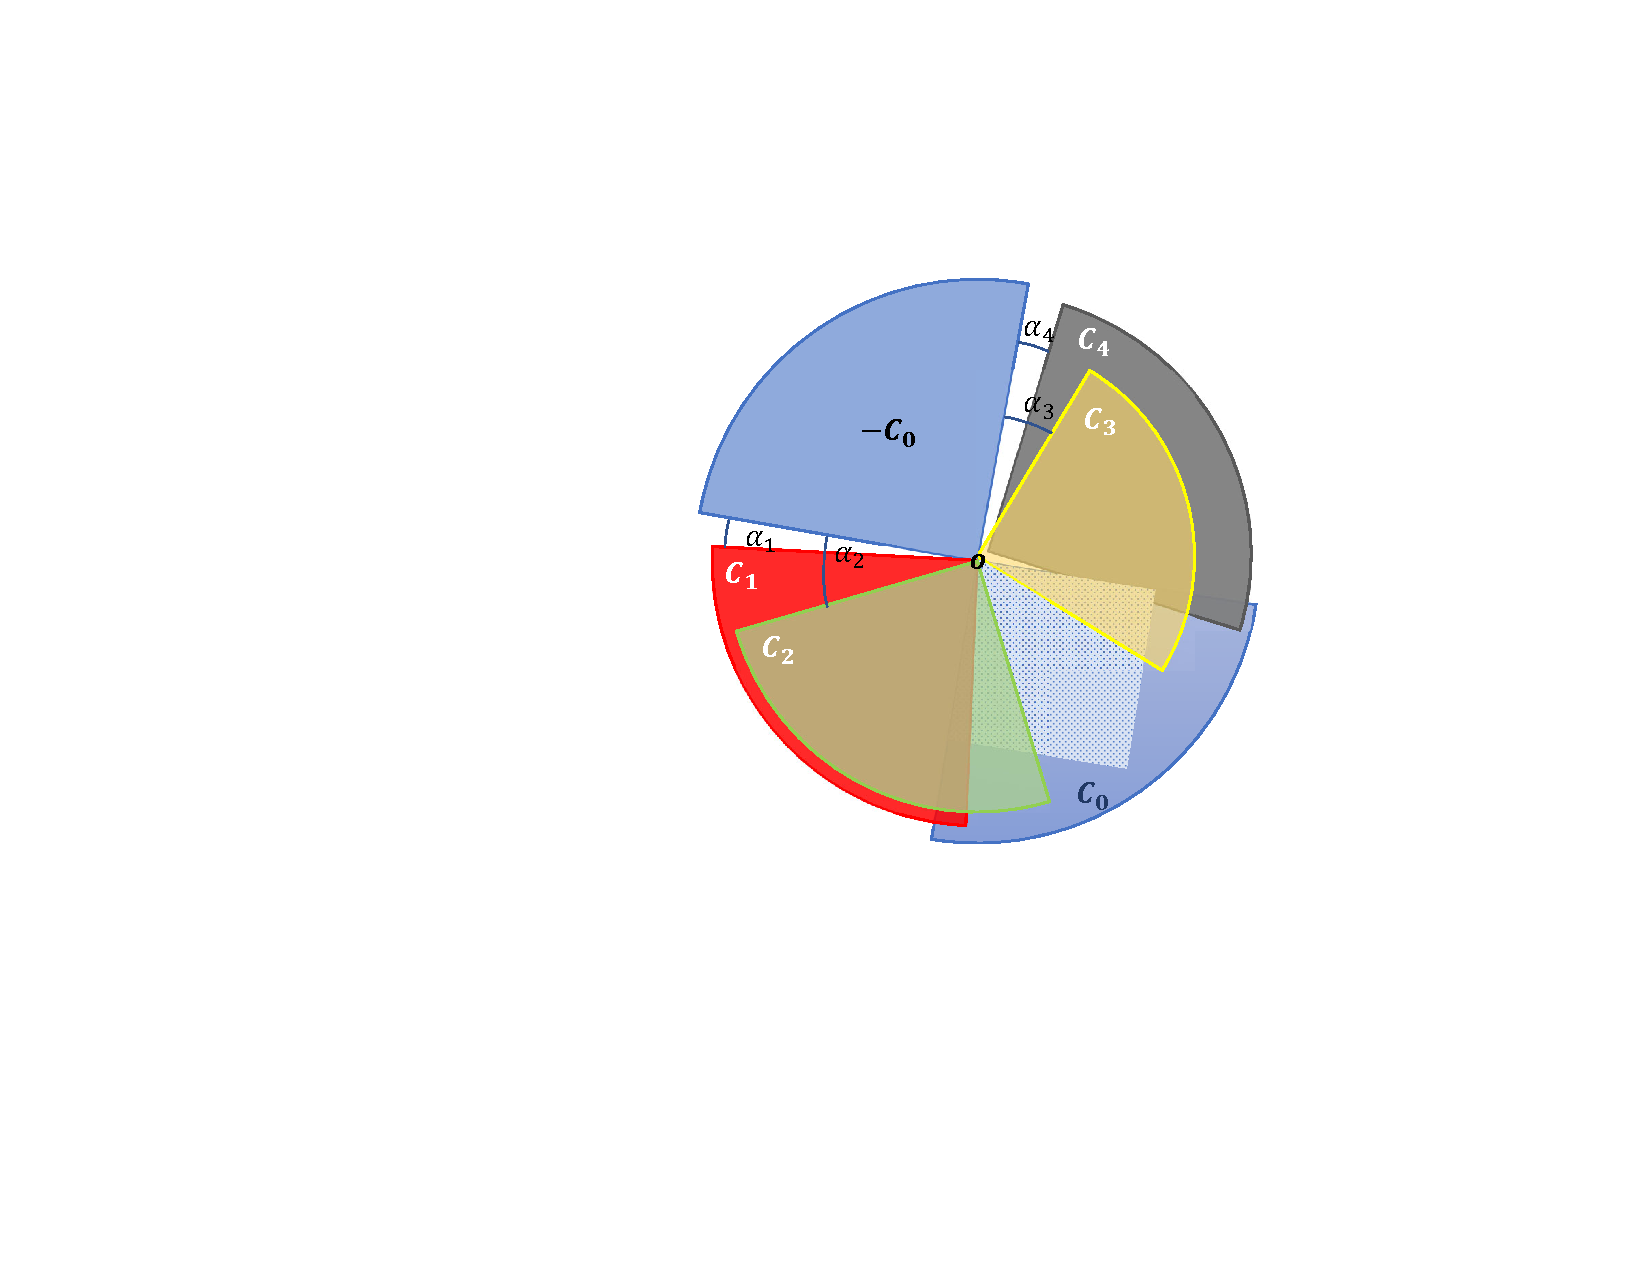
\includegraphics[width=\textwidth]{./img/sc.pdf}
		\caption{Structural Coherence (SC) condition.}\label{fig:sc}
	\end{subfigure} 
	~
	\begin{subfigure}[t]{0.43\textwidth}
		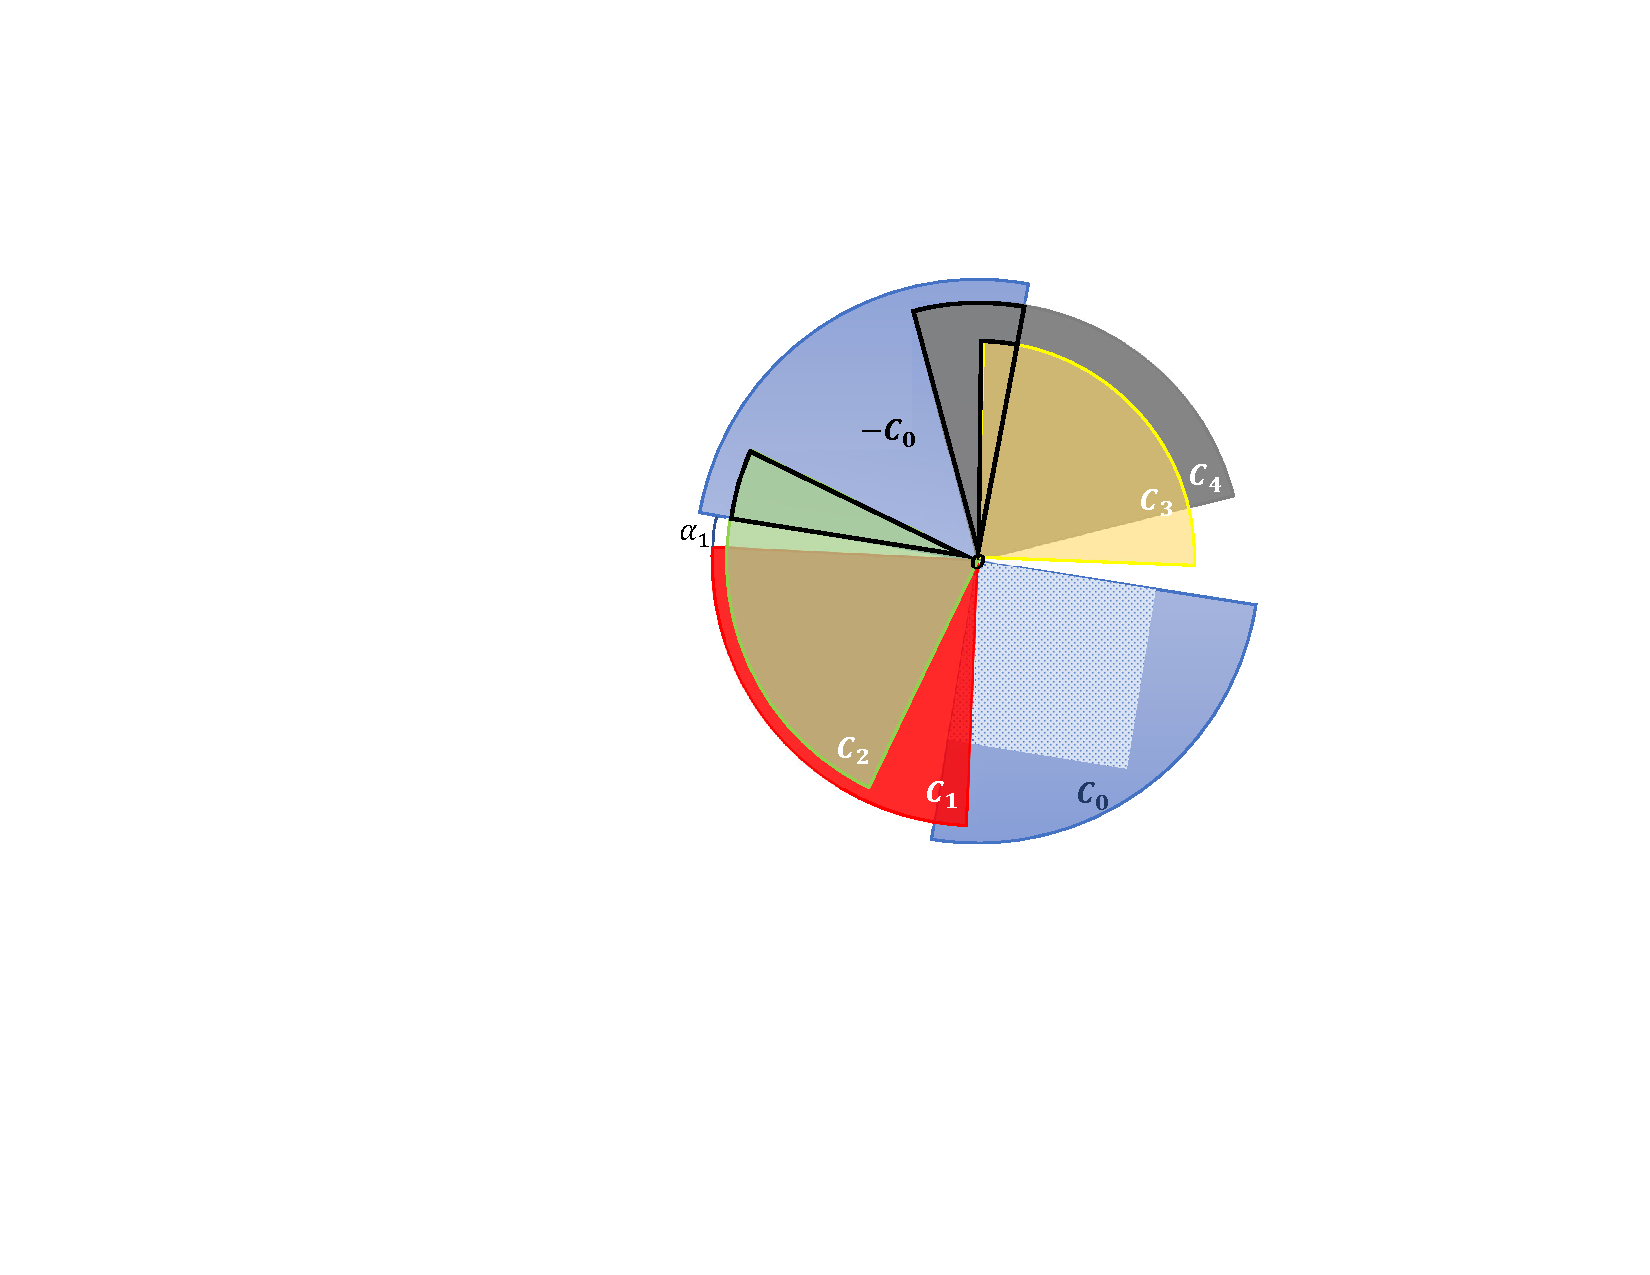
\includegraphics[width=\textwidth]{./img/deric.pdf}
		\caption{Data EnRichment Incoherence Condition (DERIC).}
		\label{fig:deric}
	\end{subfigure}
	\squeezeup
	\caption{a) State-of-the-art condition for recovering common and individual parameters in superposition models where $\cC_g = \text{Cone}(\cE_g)$ are error cones and $\cE_g = \left\{\ddelta_g | f_g(\bbeta _g^* + \ddelta_g) \leq f_g(\bbeta _g^*)\right\}$ are the error sets for each parameter $\bbeta^*_g \in [G]$ \cite{guba16}. b) Our more relaxed recovery condition which allows \emph{arbitrary non-zero fraction } of the error cones of individual parameters intersect with $-\cC_0$.}
	\label{fig syn2}
\end{figure}

